\chapter{操作系统接口}

操作系统的任务是让多个程序共享计算机,并且除了硬件已经支持的服务之外,还要提供更多有用的服务。
操作系统对底层的硬件进行管理和抽象,例如,一个字处理程序不需要关心它自己正在使用什么类型的磁盘。
它还在多个程序之间共享硬件,来让它们同时(或者看起来同时)运行。
最后,操作系统还提供可控的方式以允许程序进行交互,因此它们可以共享数据或者协同工作。

一个操作系统通过接口向用户程序提供服务。
事实证明设计一个好的接口被证明是非常困难的。
一方面,我们希望接口尽量简单和特化,因为这样可以更容易地正确实现它们。
另一方面,我们还希望向应用提供很多复杂的特性。
解决这种问题的方法是设计可以通过一些机制进行组合来提供复杂服务的简单接口。

这本书使用一个单独的操作系统作为具体的例子来展示操作系统的概念。
该操作系统,xv6,提供了Ken Thompson和Dennis Ritchie的Unix操作系统[17]中引入的基本接口,同时模仿了Unix的内部设计。
Unix提供了一个特化的接口,但它们的机制结合得非常好,提供了惊人的通用性。
这个接口如此成功,以至于现代操作系统——BSD,Linux,Mac OS X,Solaris,甚至在某种程度上,就连Microsoft Windows都有类Unix接口。
理解xv6是理解这些现代操作系统的一个好的开始。

如\autoref{f1-1}所示,xv6采用了\emph{内核(kernel)}的传统模式,内核是一个为运行中的程序提供服务的特殊程序。
每一个运行中的程序被称为一个\emph{进程(process)},它们都拥有包含指令、数据、栈的内存空间。
指令实现了程序的计算过程。
数据是计算操作时的变量。
栈用于组织程序的过程调用。
一台计算机里通常有很多进程单只有一个内核。

\begin{figure}[htbp]
    \centering
    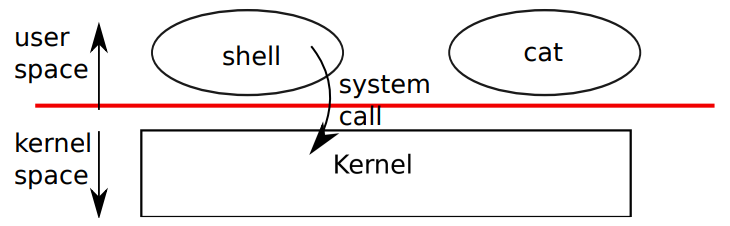
\includegraphics[width=0.8\textwidth]{../imgs/f1-1.png}
    \caption{一个内核和两个用户进程}
    \label{f1-1}
\end{figure}

当一个进程需要调用一个内核服务时,它会调用操作系统接口中的一个过程调用。
这样的过程被称为\emph{系统调用(system call)}。
系统调用会进入内核,然后内核执行服务并返回。
因此一个进程会在\emph{用户空间(user space)}和\emph{内核空间(kernel space)}中交替执行。

正如后续章节中详细介绍的那样,内核使用CPU\footnote{本书中使用术语\emph{CPU}(中央处理器的缩写)来指代执行计算的硬件。其他文档(例如RISC-V规范)中也可能使用处理器(processor)、核心(core)、hart来代替CPU。}的硬件保护机制来保证每个在用户空间执行的进程只能访问它自己的内存。
内核在执行时需要硬件特权来实现这些保护;而用户程序执行时没有特权。
当一个用户程序调用一个系统调用时,硬件会提高特权等级,然后开始执行内核中事先设置好的一个函数。

内核提供的系统调用的集合就是用户程序看到的接口。
xv6内核提供了Unix内核通常提供的服务和系统调用的一个子集。
\autoref{t1-1}列出了xv6的所有系统调用。

\begin{table}[htbp]
    \centering
    \begin{tabular}{ll}
        \textbf{系统调用}   & \textbf{介绍} \\
        int fork()  & 创建一个子进程,返回子进程的PID。\\
        int exit(int status)    & 终止当前进程;status会汇报给wait()。不会返回。\\
        int wait(int *status)   & 等待一个子进程退出;退出状态存储在*status,返回子进程的PID。 \\
        int kill(int PID)   & 终止PID进程。返回0,出错时返回-1.\\
        int getPID()    & 返回当前进程的PID。         \\
        int sleep(int n)    & 暂停\texttt{n}个时钟周期。  \\
        int exec(char *file, char *argv[])  & 加载一个文件并以给定参数执行它,只有当出错时才会返回。  \\
        char *sbrk(int n) & 将进程的内存扩大n个字节。返回新内存的起始位置。   \\
        int open(char *file, int flags) & 打开一个文件;flag指示读/写;返回一个fd(文件描述符)。 \\
        int write(int fd, char *buf, int n)   & 将从buf开始的n个字节写入到文件描述符fd中;返回n。 \\
        int read(int fd, char *buf, int n)    & 读取n个字节到buf;返回读取的字节数;或者文件结尾时返回0。 \\
        int close(int fd)   & 关闭打开的文件fd。  \\
        int dup(int fd)     & 新创建一个和fd指向同一个文件的文件描述符。    \\
        int pipe(int p[])     & 创建一个管道,并把读/写它的文件描述符存入p[0]和p[1]。 \\
        int chdir(char *dir)  & 改变当前目录。  \\
        int mkdir(char *dir)  & 创建一个新目录。    \\
        int mknod(char * file, int, int)   & 创建一个设备文件。  \\
        int fstat(int fd, struct stat *st)       & 把一个打开的文件的信息存入*st。  \\
        int stat(char *file, struct stat *st) &  把一个命名文件的信息存入*st。\\
        int link(char *file1, char *file2)    & 创建文件file1的别名file2    \\
        int unlink(char *file)& 移除一个文件。 \\
    \end{tabular}
    \caption{xv6系统调用。如果没有特殊说明,这些调用返回0表示没有错误,返回-1表示出错。}
    \label{t1-1}
\end{table}

本章的剩余部分概述了xv6的服务——进程、内存、文件描述符、管道、文件系统——并且通过代码片段对它们进行说明,并讨论\emph{shell}(Unix的命令行用户接口)如何使用它们。
shell对系统调用的使用展示了它们的设计有多么精巧。

shell是一个读取用户的命令然后执行它们的普通程序。
它是一个用户程序,不是内核的一部分。
这一事实展示了系统调用接口的强大:shell并没有什么特殊的地方。
这也意味着shell可以很容易的替换;因此,现代Unix系统有很多shell可以选择,每一个都有自己的用户借口和脚本特性。
xv6的shell是Unix Bourne Shell的基础部分的一个简单实现。
它的实现可以在\href{https://github.com/mit-pdos/xv6-riscv/blob/riscv//user/sh.c#L1}{(user/sh.c:1)}找到。

\section{处理器和内存}

一个xv6进程由用户空间内存(指令、数据、栈)和内核中私有的每个进程的状态组成。
xv6\emph{分时共享(time-share)}处理器:它在一个等待执行的进程的集合中透明地切换可用的CPU。
当一个进程不在执行时,xv6会保存它的CPU寄存器,并在下一次执行这个进程时恢复它们。
内核为每个进程关联一个进程标识符,或者叫\texttt{PID}。

一个进程可能会使用\texttt{fork}系统调用创建一个新的进程。
\texttt{fork}会给予新进程一份调用者进程的内存的拷贝,包括指令和数据。
\texttt{fork}在原进程和新进程中都会返回。
在原进程中,\texttt{fork}会返回新进程的PID;而在子进程中,\texttt{fork}返回0。
原进程和新进程通常被称为\emph{父(parent)进程}和\emph{子(child)进程}。

例如,考虑下面来自《C Programming language》[7]中的程序片段:

\begin{lstlisting}
    int pid = fork();
    if (pid > 0) {
        printf("parent: child=%d\n", pid);
        pid = wait((int *) 0);
        printf("child %d is done\n", pid);
    } else if (pid == 0) {
        printf("child: exiting\n");
        exit(0);
    } else {
        printf("fork error\n");
    }
\end{lstlisting}

\texttt{exit}系统调用会让调用者进程停止执行并释放资源,例如内存和打开的文件。
\texttt{wait}系统调用返回当前进程的一个退出的(或者被杀死的)子进程的PID,并把子进程的退出状态拷贝到传给wait的地址处;如果调用者的子进程都还没有退出,那么\texttt{wait}会等待一个子进程退出。
如果调用者没有子进程,\texttt{wait}会立刻返回-1。
如果父进程并不关心子进程的退出状态,它可以向\texttt{wait}传递0地址。

在这个例子中,会输出:
\begin{blacklisting}
    parent: child=1234
    child: exiting
\end{blacklisting}    

也可能以其他顺序输出(甚至互相交错),取决于父进程还是子进程先到达\texttt{printf}调用。
当子进程退出后,父进程的\texttt{wait}会返回,然后父进程会打印出
\begin{blacklisting}
    parent: child 1234 is done
\end{blacklisting}

尽管子进程一开始有和父进程同样的内存内容,但父进程和子进程是在不同的内存和不同的寄存器中执行:修改其中一个的变量并不会影响另一个中同名的变量。
例如,当父进程中\texttt{wait}的返回值被存储到\texttt{pid}中时,并不会修改子进程中的\texttt{pid}变量。
子进程中的\texttt{pid}仍然是0。

\texttt{exec}系统调用会把调用者进程的内存替换为从文件系统的某个文件中加载的一个新的内存镜像。
这个文件必须有特定的格式,这个格式指定了文件中哪一部分存储指令、哪一部分是数据、从哪一条指令开始执行,等等。
xv6使用ELF格式,\autoref{ch03}中将会详细介绍这种格式。
这种文件通常是编译程序源代码得到的结果。
当\texttt{exec}成功时,它并不会返回到调用者程序;而是开始执行从文件中加载的指令,执行的起点是ELF头中声明的入口点。
\texttt{exec}有两个参数:包含可执行程序的文件的名字,和一个字符串参数的数组。
例如:
\begin{lstlisting}
    char *argv[3];

    argv[0] = "echo";
    argv[1] = "hello";
    argv[2] = 0;
    exec("/bin/echo", argv);
    printf("exec error\n");
\end{lstlisting}

这个片段将调用者程序替换为\texttt{/bin/echo}程序的实例,并以\texttt{echo hello}作为参数列表。
大多数程序会忽略第一个参数,按照惯例它是程序的名称。

xv6 shell使用上面的调用来代替用户运行程序。shell的主要架构很简单,见\href{https://github.com/mit-pdos/xv6-riscv/blob/riscv//user/sh.c#L146}{(usr/sh.c:146)}。
主循环使用\texttt{getcmd}读取用户的一行输入。
然后它调用\texttt{fork},创建一个shell进程的拷贝。
父进程调用\texttt{wait},而子进程运行读入的命令。
例如,如果用户向shell输入了“\texttt{echo hello}”,\texttt{runcmd}将会以“\texttt{echo hello}”为参数被调用。
\texttt{runcmd}\href{https://github.com/mit-pdos/xv6-riscv/blob/riscv//user/sh.c#L55}{(user/sh.c:55)}运行实际的命令。
对于“\texttt{echo hello}”,它会调用\texttt{exec}\href{https://github.com/mit-pdos/xv6-riscv/blob/riscv//user/sh.c#L79}{(user/sh.c:79)}。
如果\texttt{exec}成功,那么子进程会执行来自\texttt{echo}的指令而不是\texttt{runcmd}。
在某个时间点\texttt{echo}会调用\texttt{exit},这导致父进程从\texttt{main}\href{https://github.com/mit-pdos/xv6-riscv/blob/riscv//user/sh.c#L146}{(user/sh.c:146)}中的\texttt{wait}返回。

你可能想知道为什么\texttt{fork}和\texttt{exec}不被合并成单个系统调用;我们稍后将会看到shell在实现I/O重定向时就利用了这种分离机制。如果创建一个复制进程之后立即替换它(使用\texttt{exec})会导致浪费,为了避免这种浪费,内核会通过使用虚拟内存技术例如写时复制(见\autoref{s4.6})来优化\texttt{fork}的实现。

xv6隐式分配大多数用户空间的内存:\texttt{fork}会为子进程分配内存来存储父进程内存的拷贝,\texttt{exec}会分配足够的内存来存储可执行文件。
一个进程如果在运行时需要更多的内存(可能是调用了\texttt{malloc}),可以调用\texttt{sbrk(n)}来把它的数据内存增大\texttt{n}个字节;\texttt{sbrk}返回新的内存的位置。

\section{I/O和文件描述符}

\emph{文件描述符(file descriptor)}是一个小整数,它表示一种由内核管理的对象,这种对象可能被一个进程读取或写入。
一个进程可以通过打开文件、目录、设备,创建管道,复制现有描述符来获得一个文件描述符。
为了简单,我们通常将文件描述符指向的对象称为“文件”;文件描述符接口对不同的文件、管道、设备进行了抽象,让它们看起来都像是字节流。

在内部,xv6内核使用文件描述符作为每个进程表的索引,这样每一个进程都有一个从0开始的文件描述符的私有空间。\footnote{todo!}
按照惯例,一个进程从文件描述符0(标准输入)读取输入,把输出写入到文件描述符1(标准输出),把错误消息写入到文件描述符2(标准错误)。
正如我们将看到的,shell利用这些惯例来实现I/O重定向和管道。
shell保证它总是至少有三个文件描述符是打开的(8707),默认情况下就是控制台的文件描述符。

\texttt{read}和\texttt{write}系统调用从文件描述符指定的文件中读取或写入字节。
\texttt{read(fd, buf, n)}调用从文件描述符\texttt{fd}中读取最多\texttt{n}个字节,拷贝到\texttt{buf}中,然后返回读取到的字节数。
每一个指向文件的文件描述符都有一个关联的偏移量。
\texttt{read}从文件的这个偏移量位置开始读取,然后把偏移量增大读到的字节数:后续的\texttt{read}将返回上一次\texttt{read}读到的字节之后的字节。
当没有字节可以读取时,\texttt{read}会返回0表示已经到达文件结尾。

\texttt{write(fd, buf, n)}调用把\texttt{buf}中的前\texttt{n}个字节写入到文件描述符\texttt{fd},然后返回写入的字节数。
只有当有错误发生时写入的字节数才会小于\texttt{n}。
类似于\texttt{read},\texttt{write}也从当前文件的偏移量处开始写入,然后把偏移量增大写入的字节数:每一个\texttt{write}调用都会在上一次写入的位置之后写入。

下面的程序片段(\texttt{cat}的基础部分)从标准输入拷贝数据到标准输出。如果有错误发生,它把错误写入到标准错误。
\begin{lstlisting}
    char buf[512];
    int n;
    for (;;) {
        n = read(0, buf, sizeof buf);
        if (n == 0)
            break;
        if (n < 0) {
            fprintf(2, "read error\n");
            exit();
        }
        if (write(1, buf, n) != n) {
            fprintf(2, "write error\n");
            exit();
        }
    }
\end{lstlisting}

这个代码片段中需要注意的一点是\texttt{cat}并不知道它是从一个文件、控制台还是管道中读取。
类似的,\text{cat}也不知道它是打印到控制台、文件还是别的什么。
文件描述符的使用和文件描述符0是输入、文件描述符1是输出的约定让我们有了一个\texttt{cat}的简单实现。

\texttt{close}系统调用释放一个文件描述符,让它可以被后续的\texttt{open}、\texttt{pipe}或\texttt{dup}系统调用重用。
一个新分配的文件描述符总是当前进程未使用的序号最小的描述符。

文件描述符和\texttt{fork}交互可以很容易地实现I/O重定向。
\texttt{fork}拷贝父进程的文件描述符表和它的内存,因此子进程开始时打开的文件和父进程完全相同。
系统调用\texttt{exec}替换调用者进程的内存但保留它的文件描述符表。
这允许shell通过fork、重新打开选定的文件描述符、然后执行新程序来实现I/O重定向。
这里有一个当shell运行命令\texttt{cat < input.txt}时会执行的代码的简单版本:

\begin{lstlisting}
    char *argv[2];

    argv[0] = "cat";
    argv[1] = 0;
    if (fork() == 0) {
        close(0);
        open("input.txt", O_RDONLY);
        exec("cat", argv);
    }
\end{lstlisting}

子进程关闭了文件描述符0之后,\texttt{open}会保证让新打开的\texttt{input.txt}使用文件描述符0:0是最小的可用文件描述符。
然后\texttt{cat}执行时,文件描述符\texttt{0}(标准输入)就指向\texttt{input.txt}。

xv6 shell中I/O重定向的代码就是用这种方式工作的(8630)。
回想之前shell已经克隆好子进程,\\
\texttt{runcmd}即将调用\texttt{exec}加载新程序。\footnote{todo!}
现在应该很清楚为什么说分离\texttt{fork}和\texttt{exec}是一个很聪明的设计了。
因为如果它们是分离的,shell可以fork一个子进程,然后在子进程中使用\texttt{open}、\texttt{close}、\texttt{dup}来改变标准输入和输出文件描述符,然后再调用\texttt{exec}。

最后exec的程序(我们的例子中是cat)不需要做任何的修改。
如果\texttt{fork}和\texttt{exec}被组合成单个系统调用,那么shell需要一些其他(可能更复杂)的方案来重定向输入和输出,或者程序自身必须知道如何重定向输入输出。

尽管\texttt{fork}会拷贝文件描述符表,但每一个底层的文件偏移量会被父进程和子进程共享。考虑这个例子:
\begin{lstlisting}
    if (fork() == 0) {
        write(1, "hello ", 6);
        exit();
    } else {
        wait();
        write(1, "world\n", 6);
    }
\end{lstlisting}
在这个片段的末尾,文件描述符1指向的文件将包含数据\texttt{hello world}。
父进程的\texttt{write}(因为\texttt{wait}调用,一定会在子进程完成后才会调用)会在子进程的\texttt{write}写入的位置之后写入。
这个行为可以让一个shell命令的序列的输出保持有序,例如\texttt{(echo hello; echo world) > output.txt}。

\texttt{dup}系统调用会复制一个现有的文件描述符,返回一个新的文件描述符,但是指向同一个底层的I/O对象。
两个文件描述符共享偏移量,就像\texttt{fork}复制的文件描述符一样。
这是另一种向一个文件中写入\texttt{hello world}的方法:
\begin{lstlisting}
    fd = dup(1);
    write(1, "hello ", 6);
    write(fd, "world\n", 6);
\end{lstlisting}

如果两个文件描述符通过\texttt{fork}和\texttt{dup}调用从同一个原始文件描述符派生,那么它们将共享同一个的偏移量。
否则文件描述符不会共享偏移量,即使它们是使用\texttt{open}调用打开的同一个文件。
\texttt{dup}允许shell实现类似这样的命令:\texttt{ls existing-file non-existing-file > tmp1 2>\&1}。\texttt{2>\&1}告诉shell文件描述符2是文件描述符1的复制。
存在的文件的文件名和不存在的文件导致的错误信息都会被输出到文件\texttt{tmp1}中。
xv6 shell不支持错误文件描述符的I/O重定向,但现在你知道了如何实现它。

文件描述符是一个强大的抽象,因为它们隐藏了它们连接到的东西的细节:一个进程写入到文件描述符1可能会写入到一个文件、也可能写入到一个设备例如控制台,也可能写入到一个管道。

\section{管道}
\emph{管道(pipe)}是一个暴露给进程的很小的内核缓冲区,在进程看来它是两个文件描述符,一个用于读,一个用于写。
向管道的一端写入的数据可以从管道的另一端读取出来。
管道提供了一种进程间通信的方式。

下面的示例代码运行\texttt{wc}程序,并把标准输入连接到一个管道的读取端:
\begin{lstlisting}
    int p[2];
    char *argv[2];

    argv[0] = "wc";
    argv[1] = 0;

    pipe(p);
    if (fork() == 0) {
        close(0);
        dup(p[0]);
        close(p[0]);
        close(p[1]);
        exec("/bin/wc", argv);
    } else {
        close(p[0]);
        write(p[1], "hello world\n", 12);
        close(p[1]);
    }
\end{lstlisting}

这个程序调用了\texttt{pipe},这会创建一个新的管道,并把输入和输出文件描述符记录到数组\texttt{p}中。
在\texttt{fork}之后,父进程和子进程都有指向管道的文件描述符。
子进程复制输入端到文件描述符0,然后关闭了\texttt{p}中的文件描述符,然后运行了\texttt{wc}。
当\texttt{wc}从标准输入读取时,它实际上是从管道读取。
父进程关闭了管道的输入端,向管道写入数据,然后关闭了写入端。

如果没有数据可用,对管道的\texttt{read}调用会等待有数据被写入到管道或者所有指向管道输入端的文件描述符都已经被关闭;在后面这种情况下,\texttt{read}会返回0,就像是读取到普通文件的末尾一样。
\texttt{read}会阻塞直到有新的数据到达也是子进程运行\texttt{wc}之前先把管道的写入端关闭的一个原因:如果\texttt{wc}的一个文件描述符指向管道的写入端,那么\texttt{wc}将永远不会看到文件的结果。

xv6 shell以类似上面代码的方式实现了管道符(\texttt{|})例如\texttt{grep fork sh.c | wc -l}(8650)。
子进程首先创建一个管道来连接管道符的左侧和右侧。
然后它为左侧和右侧分别调用\texttt{fork}和\texttt{runcmd},然后等待两侧都结束。
管道符的右侧可能是一个包含管道的命令(例如,\texttt{a | b | c},这时它自己还会fork两个新的子进程(一个运行\texttt{b},一个运行\texttt{c})。
因此,shell可能会创建一棵子进程树。
树的叶节点就是命令,内部的节点是等待左侧和右侧的子进程都执行结束的进程。
理论上讲,你可以让内部的节点运行管道符左侧的命令,但正确的实现这样的逻辑会让实现更加复杂。

管道可能看起来没有临时文件强大:管道
\begin{blacklisting}
    echo hello world | wc    
\end{blacklisting}
可以被实现为没有管道的版本
\begin{blacklisting}
    echo hello world >/tmp/xyz; wc </tmp/xyz
\end{blacklisting}

在这种情况下,管道相比临时文件至少有4个优势。
第一,管道会自动清理自己;而使用文件重定向,shell需要在结束之后谨慎地删除\texttt{/tmp/xyz}。
第二,管道可以传输任意长的数据流,而文件重定向需要磁盘上有足够大的空闲空间来存储所有的数据。
第三,管道运行不同阶段并行执行,而文件的方法需要第一个程序结束之后才能运行第二个。
第四,如果你在实现进程间通信,管道的阻塞读取和写入比文件的非阻塞语言更加高效。

\section{文件系统}
xv6文件系统提供数据文件,它们是未解析的字节数组;以及目录,包含指向数据文件和其他目录的名称。
目录组成一棵树,从一个称为\emph{根(root)}的特殊目录开始。
一个\emph{路径(path)}例如\texttt{/a/b/c}指向根目录\texttt{/}下的\texttt{a}目录下的\texttt{b}目录下的一个叫\texttt{c}的文件或者目录。
不以\texttt{/}开头的路径是相对于调用进程的\emph{当前目录(current directory)}的相对目录,当前目录可以通过\texttt{chdir}系统调用改变。
下面的两段代码打开同一个文件(假设涉及到的所有目录都存在):
\begin{lstlisting}
    chdir("/a");
    chdir("b");
    open("c", O_RDONLY);

    open("/a/b/c", O_RDONLY);
\end{lstlisting}
第一个片段将进程的当前目录修改为\texttt{/a/b};第二个既没有参照也没有改变进程的当前目录。

有很多系统调用来创建新的文件或者目录:\texttt{mkdir}创建一个新目录,带有\texttt{O\_CREATE} flag的\texttt{open}创建一个新的数据文件,\texttt{mknod}创建一个新的设备文件。
这个例子演示了这三个系统调用的用法:
\begin{lstlisting}
    mkdir("/dir");
    fd = open("/dir/file", O_CREATE|O_WRONLY);
    close(fd);
    mknod("/console", 1, 1);
\end{lstlisting}

\texttt{mknod}在文件系统中创建一个文件,但这个文件中没有任何内容。
这个文件的元数据标识它是一个设备文件并且记录了主设备号和次设备号(\texttt{mknod}的两个参数),内核会将读写设备的\texttt{read}和\texttt{write}系统调用自动转换为设备自身的实现,而不是文件系统的实现。

\texttt{fstat}获取一个文件描述符指向的对象的信息。它是一个\texttt{stat.h}中定义的\texttt{struct stat}:
\begin{lstlisting}
    #define T_DIR  1    // 目录
    #define T_FILE 2    // 文件
    #define T_DEF  3    // 设备

    struct stat {
        short type;     // 文件的类型
        int dev;        // 文件系统的磁盘设备
        uint ino;       // Inode号
        short nlink;    // 指向这个文件的链接数
        uint size;      // 文件的大小,单位是字节
    };
\end{lstlisting}

一个文件的名字和文件自身是不同的;同一个底层文件(称为一个\emph{i节点(inode)})可以有多个名字(称为\emph{链接(link)})。
\texttt{link}系统调用创建另一个指向同一个inode的文件系统名。
这个片段创建了一个新的文件,名字既是\texttt{a}又是\texttt{b}。

\begin{lstlisting}
    open("a", O_CREATE|O_WRONLY);
    link("a", "b");
\end{lstlisting}

读写\texttt{a}和读写\texttt{b}是一样的。
每一个i节点都由一个独一无二的\emph{i节点号(inode number)}标识。
在上面的代码片段之后,可以通过检查\texttt{fstat}的返回值来判断\texttt{a}和\texttt{b}指向相同的底层文件:它们会返回相同的i节点号(\texttt{ino}),\texttt{nlink}将会是2。

\texttt{unlink}系统调用从文件系统中移除一个名字。
只有当文件的链接数变为0并且没有文件描述符指向它时,文件的i节点和保存内容的磁盘空间才会被释放。
因此在上面的代码最后加上
\begin{lstlisting}
    unlink("a");
\end{lstlisting}
将会使i节点和文件内容只能通过\texttt{b}访问。
另外,
\begin{lstlisting}
    fd = open("/tmp/xyz", O_CREATE|O_RDWR);
    unlink("/tmp/xyz");
\end{lstlisting}
是一种惯用的创建临时i节点的方法,当进程关闭\texttt{fd}或者退出时这个i节点就会被清除。

文件系统操作的shell命令被实现为用户级的程序,例如\texttt{mkdir, ln, rm}等。
这个设计允许任何人通过添加新的用户级程序来扩展shell支持新的用户命令。
事后看来,这个设计看起来非常明显,但当时和Unix同时期的其他系统的设计通常都是把这些命令内置在shell中(并且把shell内置在内核中)。

一个例外是\texttt{cd},它被内置在shell中(8716)。
\texttt{cd}必须改变shell自身的当前工作目录。
如果\texttt{cd}作为普通的命令运行,那么shell会fork一个子进程,子进程会运行\texttt{cd},然后\texttt{cd}会改变\emph{子进程}的工作目录。
父进程(即shell)的工作目录并不会改变。

\section{现实世界}
Unix的“标准”文件描述符、管道和操作它们的便捷shell语法的组合是编写通用可重用程序的一大进步。
这个想法引起了“软件工具”的文化,这是Unix强大和流行的根本原因,shell也是第一个所谓的“脚本语言”。
Unix系统调用接口一直持续到现在的系统中,例如BSD、Linux和Mac OS X。

Unix系统调用接口通过可移植操作系统接口(Portable Operating System Interface, POSIX)标准化。
xv6\emph{不是}POSIX兼容的。
因为它缺少了很多系统系统调用(包括最基本的一些,例如\texttt{lseek}),它只实现了系统调用的部分功能等。
我们设计xv6的主要目的是简单和清晰的同时提供一个简单的类UNIX系统调用接口。
一些人给xv6扩展了一些基本的系统调用和一个简单的C库,以便可以运行基本的Unix程序。

然而,现代的内核提供的系统调用和内核设备的种类要比xv6多很多。
例如,它们支持网络,窗口系统,用户级别线程,很多设备的驱动,等等。
现代内核还在持续而快速地进化,并且提供很多POSIX之外的特性。

在大多数情况下,现代的Unix派生操作系统并没有遵循早期Unix把设备作为特殊文件暴露的模型,例如上面讨论过的\texttt{console}设备。

Unix的作者们正在构建Plan 9,它对现代设施应用“资源即文件”的概念,把网络、图形和其他资源表示为文件或者文件树。

文件系统抽象是一个强大的思路。
即使如此,操作系统接口还有很多其他的模型。
Unix的一个前辈Multics把文件存储抽象为一种类似于内存的方式,产生了一套有很大不同的接口。
Multics设计的复杂性直接影响到了Unix的设计者,他们尝试构建一些更简单的模型。

这本书解释了xv6如何实现它的类Unix接口,但思路和概念并不仅仅适用于Unix。
任何操作系统都必须复用底层的硬件,将进程彼此隔离,并且提供受控制的进程间通信机制。
在学习了xv6之后,你应该能看一看更复杂很多的操作系统,并且能在那些系统里看到和xv6的底层概念。
